\chapter{Background}\label{chp:background} 
\chapterprecishere{"We model the future on the past. Sometimes that’s a mistake."\par\raggedleft--- \textup{Van Jacobsen}, SIGCOMM 2001}

This chapter will give a brief overlook of the motivation for \gls{ICN},
as well as explaining more details of how \gls{ICN} protocols, such as \gls{CCN} and \gls{NDN}, works. 
It will also contain a quick summary of related works.

\section{Motivation for Information-Centric Networking}
When Internet was created in the 1960's, the researchers where inspired by the existing communication network, the telecommunication network.
Because it was not natural and logical to think that people would download content, but rather send and receive short messages and instructions, the point-to-point communication model was a logical architecture. 
As Internet have developed, the traffic has increased enormously over the past few years. 
In the Global Internet Phenomena Report 1H2014 done by Sandvine~\cite{gipr2014}, close to 64\% of all \gls{IP} traffic in North America was Real-Time Entertainment streaming. 
In~\autoref{fig:ip-traffic} it can easily be seen that most of the traffic is content, and not communication.
With this in mind, the \gls{IP} architecture does not provide an efficient transport model for what we are actually using the network for.

\begin{figure}[ht]
  \centering
  \begin{subfigure}{0.48\textwidth}
    \centering
    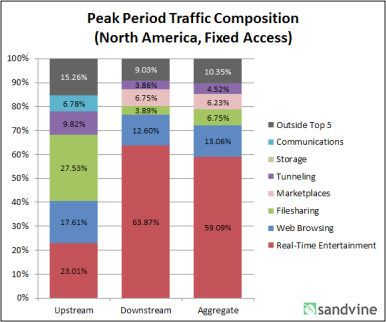
\includegraphics[width=1\linewidth]{north-america-ip-traffic.png}
    \caption{North America}
    \label{fig:north-america-ip-traffic}
  \end{subfigure}

  \begin{subfigure}{0.48\textwidth}
    \centering
    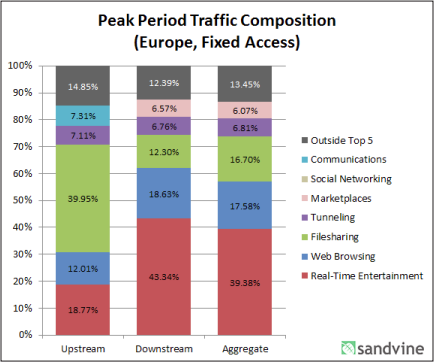
\includegraphics[width=1\linewidth]{europe-ip-traffic.png}
    \caption{Europe}
    \label{fig:europe-ip-traffic}
  \end{subfigure}
  \caption{
  (a) Peak Period Aggregate Traffic Composition - North America, Fixed Access~\cite{gipr2014}.
  (b) Peak Period Aggregate Traffic Composition - Europe, Fixed Access~\cite{gipr2014}.
  }
  \label{fig:ip-traffic}
\end{figure}

Also, the \gls{IP} network was not designed with security in mind. 
Most of the protocols related to Internet have been designed and deployed mainly with the goal of functionality to work.
\gls{IPsec} is a very good example of work trying to patch up security flaws in Internet.

A node in a \gls{IP} network does not know WHAT goes through, but rather the packet's endpoints, i.e. WHERE it goes and WHERE it comes from. 
This makes every node dumb, hence the network is designed for redundancy when it comes to content download.

\gls{TCP}/\gls{IP} not designed for broadcast and therefore wireless connection is not as easy as it can be.

These design failures are some the reasons why the research for Future Internet began.  
\gls{ICN}~\cite{DBLP:journals/cm/AhlgrenDIKO12} is a concept developed under this research.
It is built upon delivery of content, rather than the point-to-point model we previously have seen.
\gls{ICN}s goal is to build an infrastructure of a new Internet that can achieve efficient, secure and reliable distribution of content.
In 2012 \gls{IRTF} established \gls{ICN} working group.


\section{Content Centric Network \& Named Data Network}\label{chp2:sec:icn}
The first network protocol purposed for \gls{ICN}, \gls{CCN}, was presented by Van Jacobsen at Google Talk in 2006. 
He, amongst other contributors of \gls{CCN}, has been working on developing the Internet as we know since the early start.
Jacobsen has contributed to \gls{TCP}/\gls{IP}, i.e. with his flow control algorithms and \gls{TCP} header compression. 

\gls{CCN} focuses on naming content, instead of naming \gls{IP}-addresses. 
The research project is lead by \gls{PARC}.

A branch of \gls{CCN} is the \gls{NDN}~\cite{DBLP:journals/ccr/0001ABJcCPWZ14} research project started in 2010.
One of the biggest contributers is \gls{UCLA}, with Lixia Zhang in the lead. 
The \gls{NDN} project is also one of few projects selected by \gls{NSF} \gls{FIA} program~\cite{nsf-fia}.

\section{NDN Architecture}\label{chp2:sec:ndn_architecture}
Since the knowledge of how \gls{NDN} works is not disseminated amongst computer scientists, it is essential for this paper to describe how it works.
This section will describe the basic architecture of \gls{NDN}~\cite{NDN-0021} and compare some solutions with the equivalent solutions in \gls{IP}.

\subsection{Names}\label{name}
In the \gls{NDN} network there is no strict rules for a Name.
This means that a network node only routes an Interest based on longest prefix match.
Naming is left to the application design, thus it can be customized for the applications best purpose.
However the network assumes hierarchical structured names, hence it will perform better with a hierarchical name design.

For the network to perform even better, the Interest can append some Selectors that can help the network to decide which Data to retrieve and where to route.
With Selectors a partially known name can successfully retrieve the right Data.
E.g. when a user want to download the newest version of some content, lets say ``/ndn/no/ntnu/haakon/file/<version?>'', but do not know which version is the newest, the user can append a ChildSelector to choose the greatest version.

When designing applications for the \gls{NDN} network, one might learn from \gls{DNS} and \gls{OS} naming.

\subsection{Packets}\label{packets}
There is two types of packets in \gls{NDN};
\textit{Interest packet} and the corresponding answer, i.e. the \textit{Data packet}, illustrated in~\autoref{fig:packets}.

\begin{figure}[H]
  \centering
  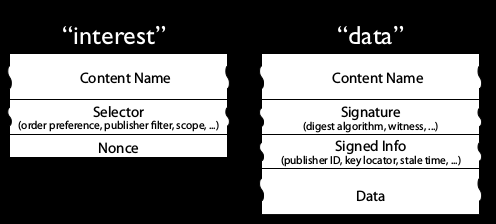
\includegraphics[width=1\textwidth]{packets.png}
  \caption{Interest packet and Data packet}
  \label{fig:packets}
\end{figure}

The Interest packet specifies a Content Name. 
The name can have a hierarchical structure and signatures can be added after the \gls{URI}, e.g. ``/ndn/no/ntnu/haakon/file/1/<signature>''.
An Interest can also contain a set of different Selectors to specify original requirements for the Data response. 
Some of the Selector fields are:
\begin{itemize}
  \item KeyLocator - can be used to specify where the Public Key for the signature can be found.
  \item Exclude - can be used to specify a list or a range of names that should be excluded from the Name. 
  I.e. if the Name is ``/ndn/no/ntnu'' and the Exclude contains ``/item'', the returned Data does not contain ``/ndn/no/ntnu/item''.
  \item MustBeFresh - if True, a node cannot answer with a Data packet where the FreshnessPeriod has expired.
  \item ChildSelector - can be used to select either the leftmost (least) or the rightmost (greatest) child, e.g. content version. 
  \item Min/MaxSuffixComponents - refers to name components that occur in the matching Data beyond the prefix. 
\end{itemize}
The Nonce field sets automatically. 
This is used to uniquely identify an Interest and prevent looping in the network.

The Data packet it a response to the Interest packet, and contains the Content Name and the Content itself.
It also has a MetaInfo field that is used to specify the FreshnessPeriod (milliseconds), ContentType and FinalBlockId. 
Now when somebody requests a file ``/ndn/no/ntnu/haakon/file/1'' with an Interest, the response will have the same name, but also containing the file.

Because only a Data packet can exists if there is a corresponding Interest, \gls{NDN} is pull-based.
Hence unsolicited Data packets will be thrown away, i.e. there is no content in the network, that is not requested from someone.
This reduces unwanted traffic compared to \gls{UDP} in \gls{IP}.

\subsection{Network Node}
If we look at an existing model of an \gls{IP} node~\autoref{fig:ip-model-node} and compare it to a \gls{NDN} node~\autoref{fig:icn-model-node}, we see that they look much the same.
However, the logic behind a \gls{NDN} node is a bit more complex, thus lead to more knowledge about WHAT content the node has to offer.
To understand this, the following entities in a \gls{NDN} node should be understood:
\begin{enumerate}\label{ndn-node-modules}
  \item Face - A term used for generalization of different interfaces, e.g. physical like Ethernet, or overlay like \gls{TCP} and \gls{UDP}. A Face can also be a UNIX-domain socket for communication with a local application.
  \item \gls{PIT} - All pending or recently satisfied Interests are stored here, together with the incoming and outgoing Face.
  If a new incoming Interest matches a entry in the \gls{PIT}, the incoming Face will be added to the entry. 
  \item \gls{CS} - When a node receives a Data packet that has a corresponding entry in the \gls{PIT}, it stores the Data packet as long as possible in the \gls{CS}. 
  \item \gls{FIB} - Here a forwarding strategy is stored for each Name prefix. 
  When a node forwards an Interest, it will do a longest prefix lookup in the \gls{FIB} and send the Interest further to the best matching Face.
\end{enumerate}

\begin{figure}[H]
  \centering
  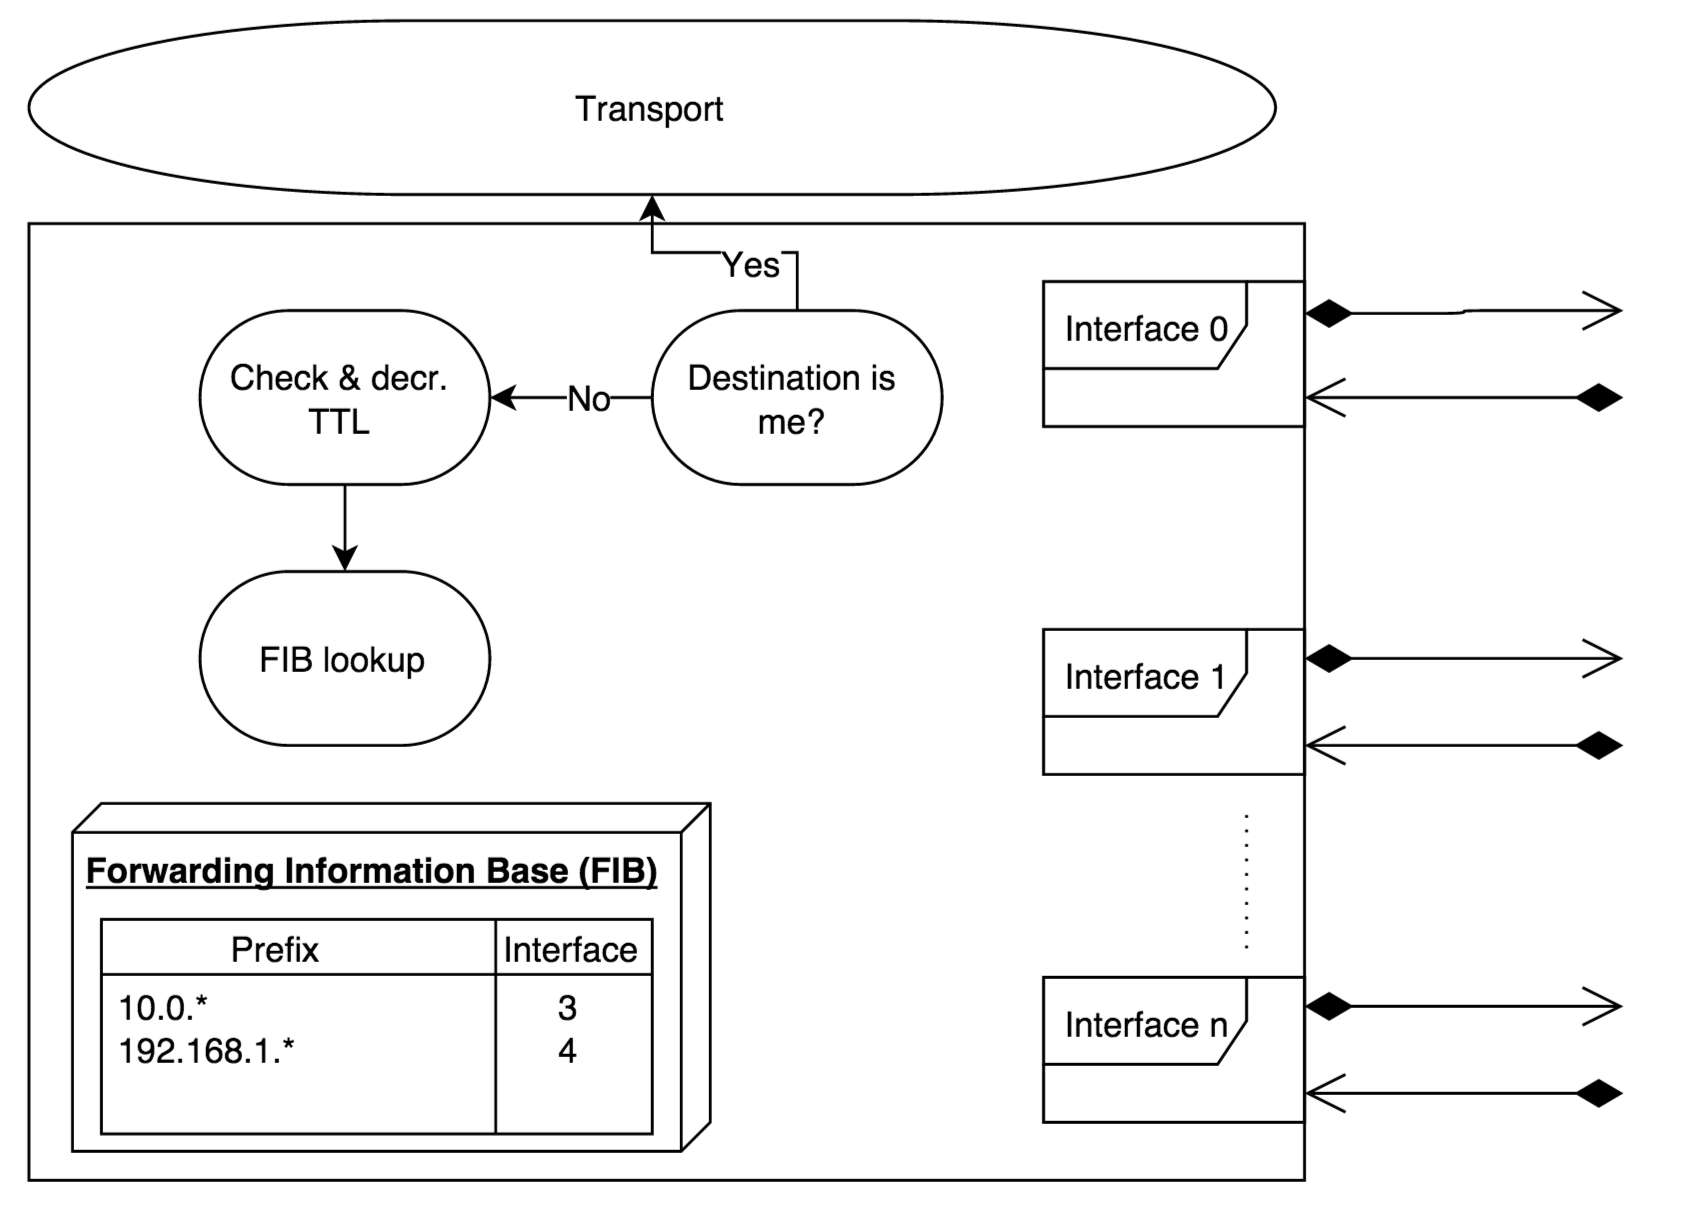
\includegraphics[width=0.8\textwidth]{ip_model_node.png}
  \caption{Model of IP node. A packets enters the node through an Face. 
  The node decides whether the packet is for the node itself, or passes it further to next node, found in the FIB.}
  \label{fig:ip-model-node}
\end{figure}

\begin{figure}[H]
  \centering
  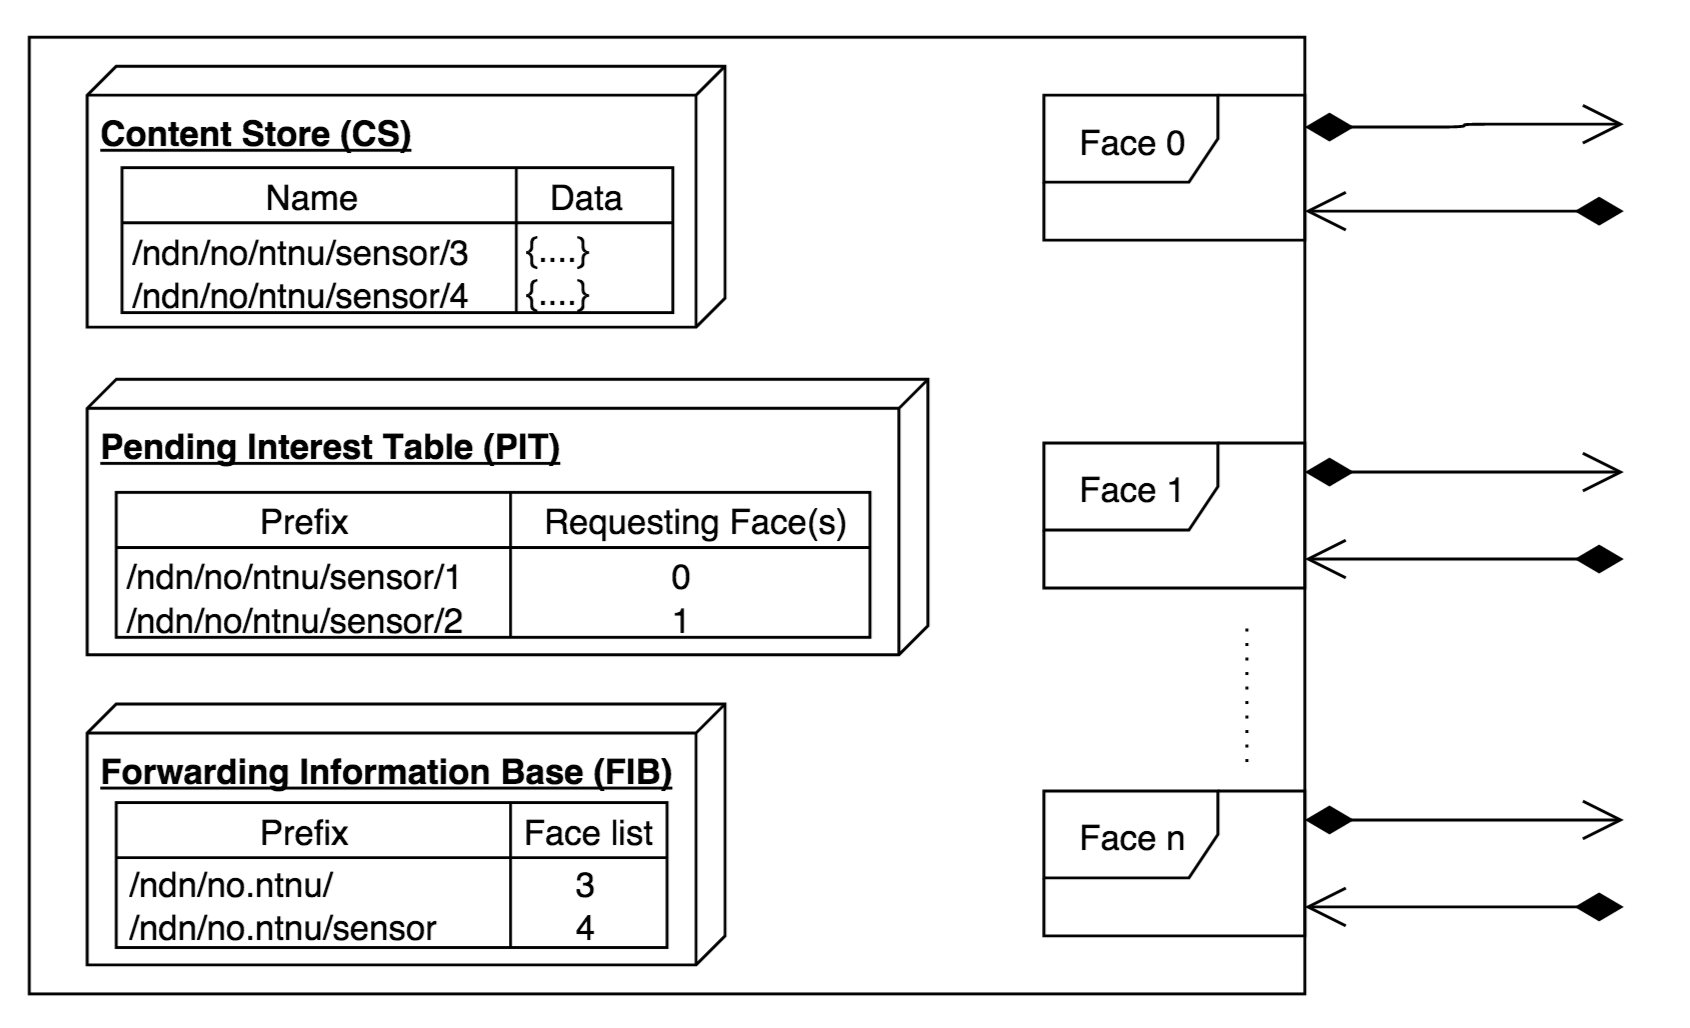
\includegraphics[width=0.8\textwidth]{icn_model_node.png}
  \caption{Model of NDN node. A packet enters through an Face. 
  The node checks whether the Interest is already queried in the PIT, or stored in the CS, or passes it further to next node, found in the FIB.}
  \label{fig:icn-model-node}
\end{figure}

In contrary to an \gls{IP} node, a \gls{NDN} node knows WHAT content comes through itself. 
Since all content is associated with a Name, a \gls{NDN} node can know 
\begin{description}
  \item[WHAT] is requested, but not satisfied (i.e. \gls{PIT})
  \item[WHAT] has been satisfied earlier, and still available (i.e. \gls{CS})
\end{description}

Unicast (TcpFace, UdpFace) vs Multicast (MulticastUdp, Ethernet)
This leads to multicast by nature.
In~\autoref{fig:ndn-multicast} we can see that the network does not nearly have to send equal amount of traffic if every node is a \gls{NDN} node.
\begin{figure}[H]
  \centering
  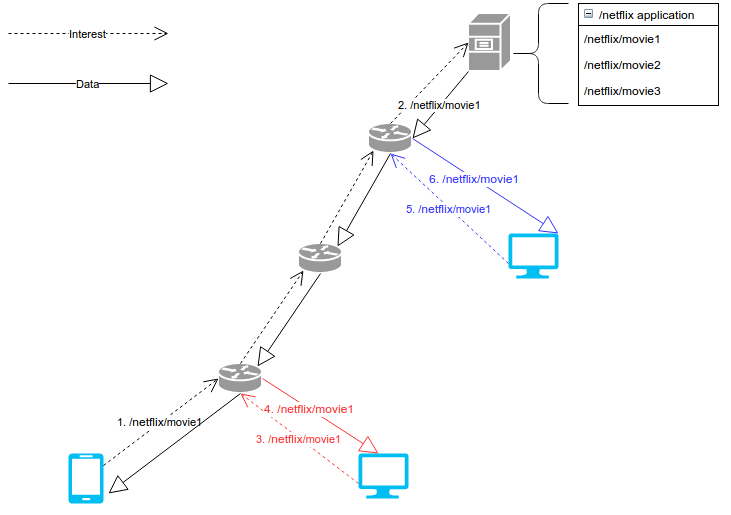
\includegraphics[width=1\textwidth]{ndn-multicast.png}
  \caption{Multicast in NDN.}
  \label{fig:ndn-multicast}
\end{figure}
 
\subsection{Incoming Interest}\label{incoming-interest}
In~\autoref{fig:icn-model-node-decision-interest} we see an incoming Interest.
Incoming Interest through a Face. The node checks the \gls{PIT} for pending or recently satisfied Interests. 
If there is no match, the node will do a lookup in \gls{CS} to see if a corresponding Data packet is cached. 
If there is a match in the \gls{PIT} it will only add the Face to the \gls{PIT} entry. If there is a match in the \gls{CS} the node will return the Data. 
If there is no match in either the \gls{PIT} or the \gls{CS} the node will make a new \gls{PIT} entry and do a longest prefix match lookup in the \gls{FIB} to decide which Face(s) to forward the Interest. 
How to forward a Interest; routing strategy. 
A strategy per \gls{PIT} entry. 
I.e. whether, when, and where to forward Interest.
\begin{figure}[H]
  \centering
  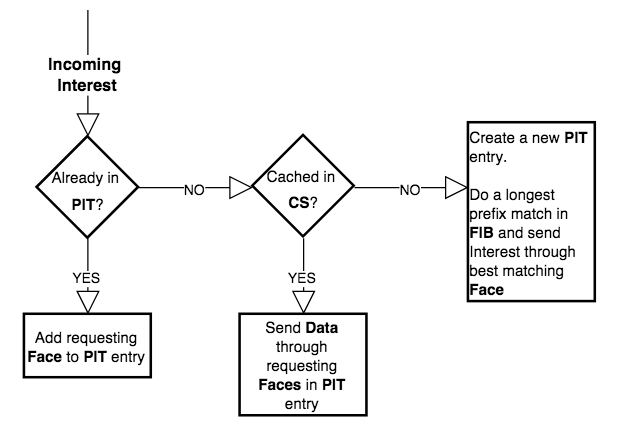
\includegraphics[width=1\textwidth]{ndn-node-decision-tree-interest.png}
  \caption{Decision tree for a NDN node when receiving an Interest.}
  \label{fig:icn-model-node-decision-interest}
\end{figure}

\subsection{Incoming Data}
In~\autoref{fig:icn-model-node-decision-data} we see incoming Data.
The node will check  the \gls{PIT} for an entry, if match it will forward the data to all the Faces registered in the \gls{PIT} entry.
Check data from local applications first cached in \gls{CS}, if not, store in \gls{CS} send data to all requesters (i.e. all Faces stored in the \gls{PIT} entry).
\begin{figure}[H]
  \centering
  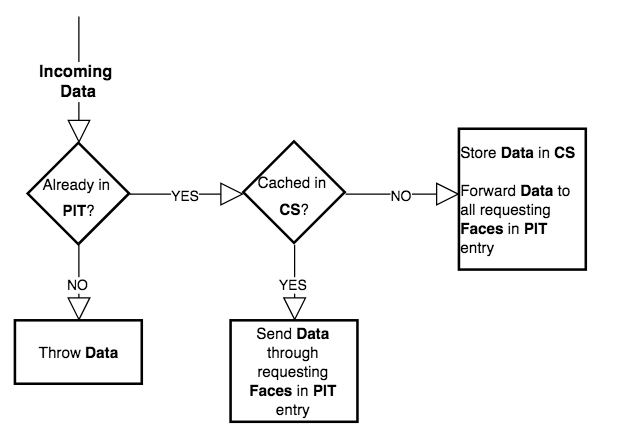
\includegraphics[width=1\textwidth]{ndn-node-decision-tree-data.png}
  \caption{Decision tree for a NDN node when receiving Data.}
  \label{fig:icn-model-node-decision-data}
\end{figure}


\subsection{Security}\label{ndn-security}
The security aspects of \gls{NDN} network protocol is one of the most important reasons why 
Secure data VS secure channel.
The network demands that every packet delivered from application layer is signed by the application for integrity and authenticity.

Based on the nature of this architecture, \gls{NDN} facilitates the practice of anonymity in the network. 
In a Tor network~\cite{DBLP:conf/uss/DingledineMS04}, each node participating in a circuit only knows the two neighboring nodes.
Only a ``Global passive adversary'' that can monitor the whole network is able to decide the whole packet path, hence know \textit{who} is requesting and \textit{who} is responding.
Since the packet format (\autoref{packets}) in \gls{NDN} has no source or destination specific field as in a \gls{IP} packet, the privacy of the network is more similar to a Tor network.
If a packet is captured at any arbitrary point of its path, the only information an adversary will get, is the two nodes between the packet capture and the data name. Unless monitoring a complete network, it should be close to impossible to track packets.  
However because of the semantic naming there are some issues related to privacy as it easily can be seen in the Name \textit{what} the content contains in many cases.
Also since signing of each Interest is required by the sender, some privacy information might leak.
DiBenedetto et al. try to address these problems in~\cite{DBLP:conf/ndss/DiBenedettoGTU12} with an approach that use existing solutions from the Tor network.

\section{Attacks}

Paolo Gasti et al. identifies several \gls{DoS} attacks on \gls{NDN} in their paper about \gls{DoS} \& \gls{DDoS} in \gls{NDN} ~\cite{DBLP:conf/icccn/GastiTU013}. Other works have been done related to \gls{DoS} in \gls{NDN}~\cite{DBLP:journals/ijcomsys/WangCZQZ14, DBLP:conf/ancs/SoNO13, DBLP:journals/corr/abs-1303-4823}

In~\cite{DBLP:journals/tifs/LiZZSF15} Zhang et al. proposes an extension of the \gls{NDN} protocol for addressing the access problem of cached data in nodes.  
The \gls{NDN} network is also potentially susceptible to content poisoning attacks which Ghali et al. addresses in~\cite{DBLP:journals/ccr/GhaliTU14}.

\section{Related work}
Synchronization application over \gls{NDN} called iSync~\cite{DBLP:conf/acmicn/FuAC14}.
A synchronization application build by the \gls{NDN} team is ChronoSync~\cite{DBLP:conf/icnp/ZhuA13}.

Amadeo et al.~\cite{DBLP:conf/acmicn/AmadeoCM14} proposes a solution for reliable retrieval of data from different wireless producers which can answer to the same Interest packet. This is highly applicable to a sensor network where you want to communicate with closest sensor, e.g. the light in \textit{this} room.
In~\cite{DBLP:conf/noms/AbidySLF14} Abid et al. simulate data aggregation in wireless sensor networks.
Burke et al. addresses efficient and secure Sensing over \gls{NDN} in~\cite{DBLP:conf/nca/BurkeGNT14}

There is done some research with \gls{IBC} in \gls{NDN}. In~\cite{DBLP:conf/icnp/ZhangCXWSW11} Zhang et al. proposes a hybrid scheme with traditional \gls{PKI} and \gls{IBC}.